\documentclass{article}

\usepackage{color}
\usepackage{hyperref}
\usepackage{pdfpages}
%\usepackage{fontawesome}

\title{\bf Student Krylov Day 2015}
\author{\href{http://sscdelft.github.io/activities/2015/02/02/krylov-day.html}{SIAM Student Chapter Delft}}
\date{February 2, 2015}
\begin{document}
\maketitle
\begin{figure}[h]
 \centering
 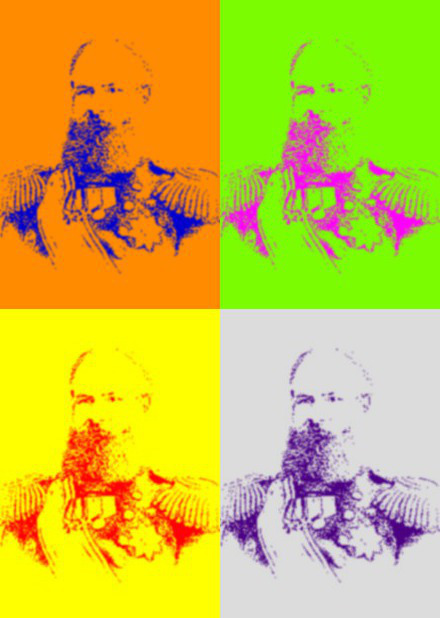
\includegraphics[width=0.5\textwidth]{krylov_warhol2.jpg} 
%  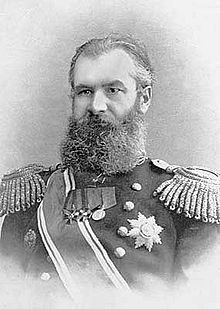
\includegraphics{220px-Alexey_Krylov_1910s.JPG}
\end{figure}

\section*{Preface}
Krylov subspace methods have been applied successfully to solve various problems 
in Numerical Linear Algebra. The Netherlands have been a pioneer country in the development of Krylov methods over the past years.
Methods like the Conjugate Gradient Squared (CGS), Bi-Conjugate Gradient Stabilized (BiCG\-STAB), Nested GMRES (GMRESR), and the Induced Dimension Reduction method (IDR) are examples of Krylov methods developed at Dutch universities. In this context, we are proud to welcome Peter Sonneveld as invited speaker to our workshop.
We are organizing the Student Krylov Day 2015 at TU Delft in the framework of the SIAM Student Chapter Delft. 
\newpage
\thispagestyle{empty}
\null
\vfill
\noindent \textbf{Sponsors:}

\begin{figure}[h]
 
\includegraphics[scale = 0.35]{Society_for_Industrial_and_Applied_Mathematics_(logo).png} \hfill
 
\includegraphics[scale = 0.75]{TU_cropped} \hfill
 
\includegraphics[scale = 0.65]{SIAMSC_Delft_cropped.png}
\end{figure}
\vspace{1cm}
\noindent \copyright \ SIAM Student Chapter Delft. All rights reserved.
\newpage
\section*{Program}
The Student Krylov Day takes place on February 2nd, 2015 at Technische Universiteit Delft, 
    Faculteit Elektrotechniek, Wiskunde en Informatica. We meet at \textbf{Snijderszaal LB 01.010.}
Mekelweg 4, 2628 CD Delft, The Netherlands. \\ 
\begin{table}[h]
\begin{tabular}{lll}
10:00 - 10:10 &  & Welcoming \\ [0.5ex]
10:10 - 10:50 & P. Sonneveld & IDR-CGS-BiCGSTAB-IDR(s) \\
 & & - a case of serendipity -\\ [0.5ex]
\hline \\ [-1.5ex]
11:00 - 11:20 & Manuel & Krylov methods for shifted linear systems \\ [0.5ex]
11:20 - 11:40 & Xian-Ming & Recent progresses in Krylov subspace methods\\ 
                        & & for solving complex symmetric linear systems\\  [0.5ex]
11:40 - 12:00 & Ian & Krylov and Matrix Balancing for fast Field \\ 
              &     & of Value Type Inclusion Regions\\  [0.5ex]
& & \hfill \small{Chairman: Reinaldo }  \\
\hline \\ [-1.5ex]
12:00 - 13:30 & & Lunch at TU Delft Sports Center \\ [0.5ex]
\hline \\ [-1.5ex]
13:30 - 13:50 & Heiko & Preconditioning of Large-Scale Saddle Point \\
                    & & Systems for Coupled Flow Problems\\ [0.5ex]
13:50 - 14:10 &J\"orn & A Krylov Subspace Approach to Modeling of \\
                     & & Wave Propagation in Open Domains\\ [0.5ex]
14:10 - 14:30 & Jing & A conjugate gradient based method for \\
                   & & frictional contact problems\\ [0.5ex]
& & \hfill \small{Chairman: Tom{\'a}{\v s}} \\
\hline \\ [-1.5ex]
15:00 - 15:20 & Tom{\'a}{\v s} & On the numerical behaviour of the CG method\\ [0.5ex]
15:20 - 15:40 & Patrick & Krylov subspace methods for matrix equations \\
                  & & which include matrix functions\\ [0.5ex]
15:40 - 16:00 & Ana & On Low-rank Updates of Matrix Functions\\ [0.5ex]
& & \hfill \small{Chairman: Heiko}  \\
\hline \\ [-1.5ex]
16:30 - 16:50 & Reinaldo & Induced Dimension Reduction method \\
            & & to solve the Quadratic Eigenvalue Problem \\ [0.5ex]
16:50 - 17:10 & Mario & Rational Least Squares Fitting using Krylov Spaces\\ [0.5ex]
17:10 - 17:30 & Sarah & Probabilistic bounds for the matrix condition  \\
                    & & number with extended Lanczos bidiagonalization\\ [0.5ex]
& & \hfill \small{Chairman: Manuel}\\
\hline \\ [-1.5ex]
17:30 - 18:30 & & Snacks \& drinks at TU Delft
\end{tabular}
\end{table}

In the evening we will go to \href{http://www.sanmarco.nl/pizzeria/}{San Marco} (Brabantse Turfmarkt 23, 2611 CL Delft). This is a nice restaurant close to the main train station. Everybody is welcome to join!

%\null\vfill\eject\thispagestyle{empty}\null\vfill\eject 
% \newpage
% \section{Book of abstracts}
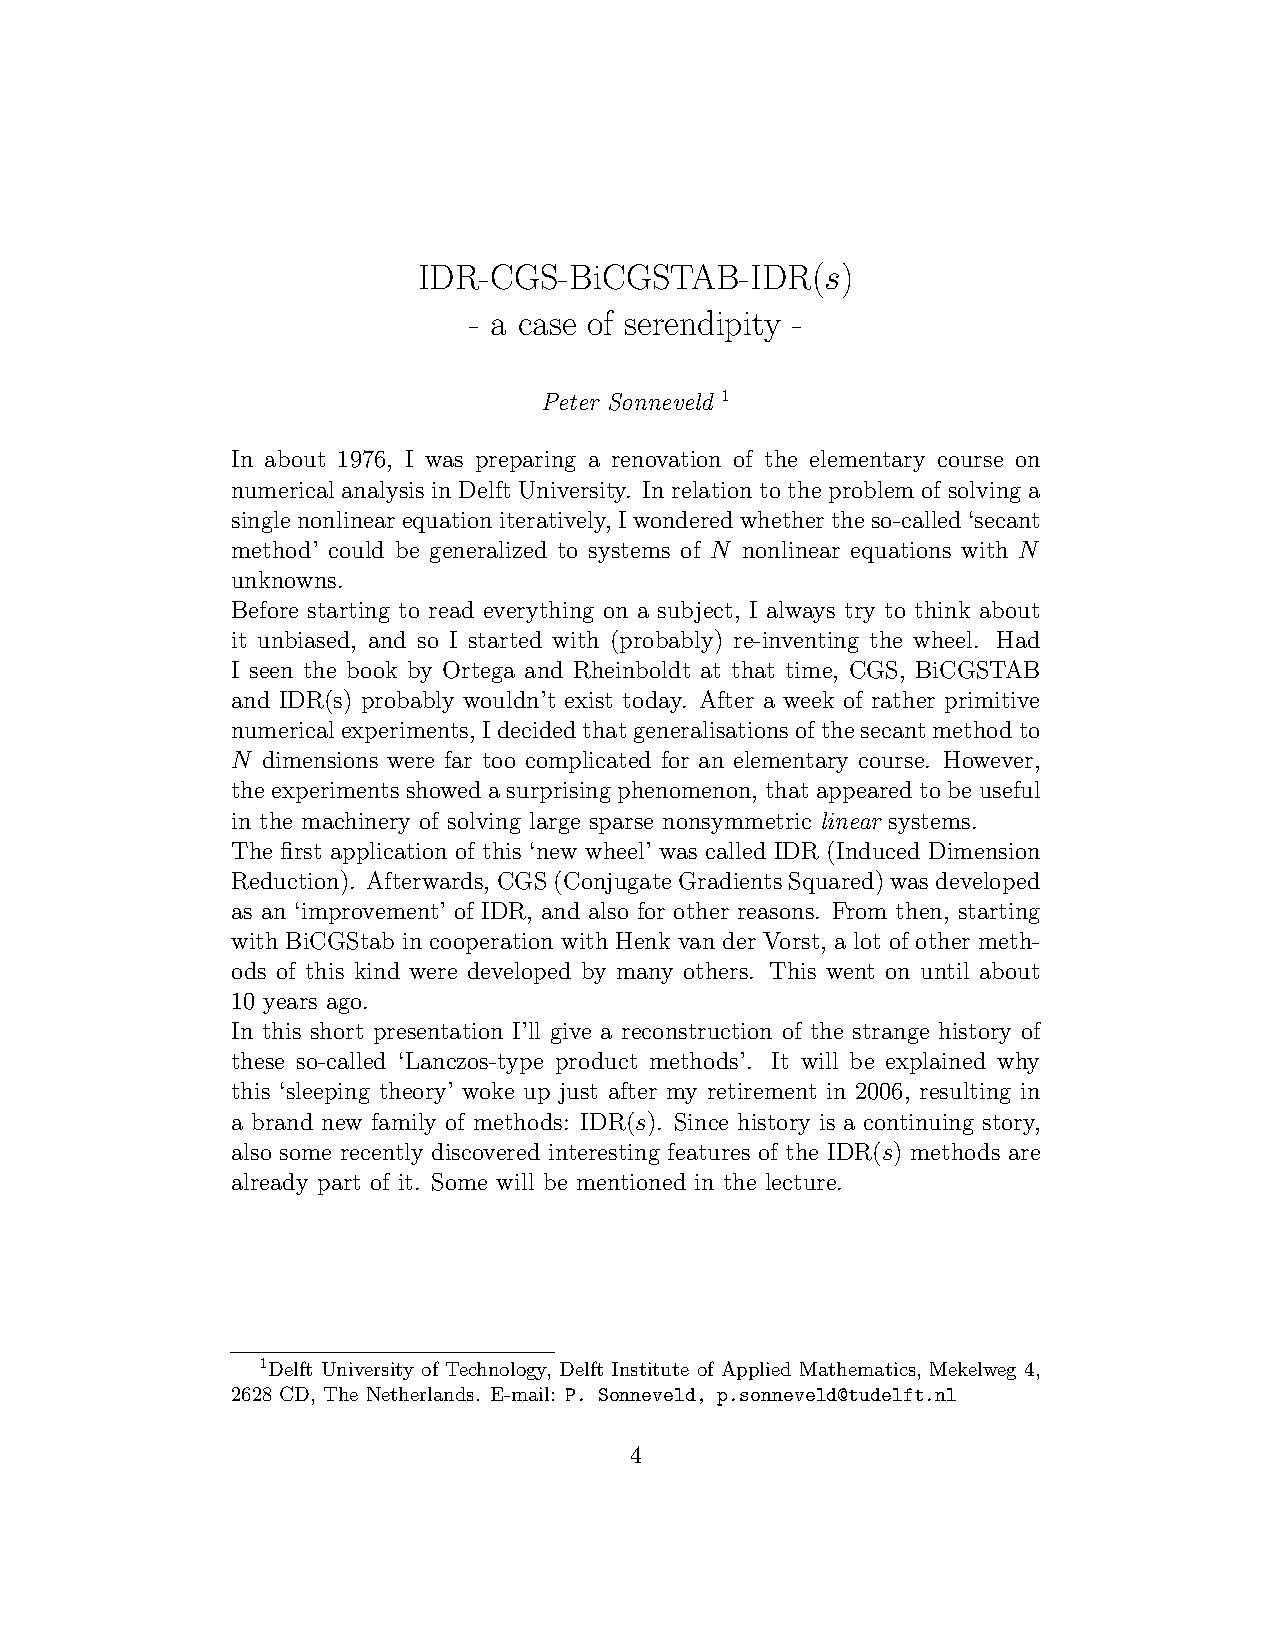
\includepdf[pages={1}]{abstracts/Summary_Sonneveld.pdf}
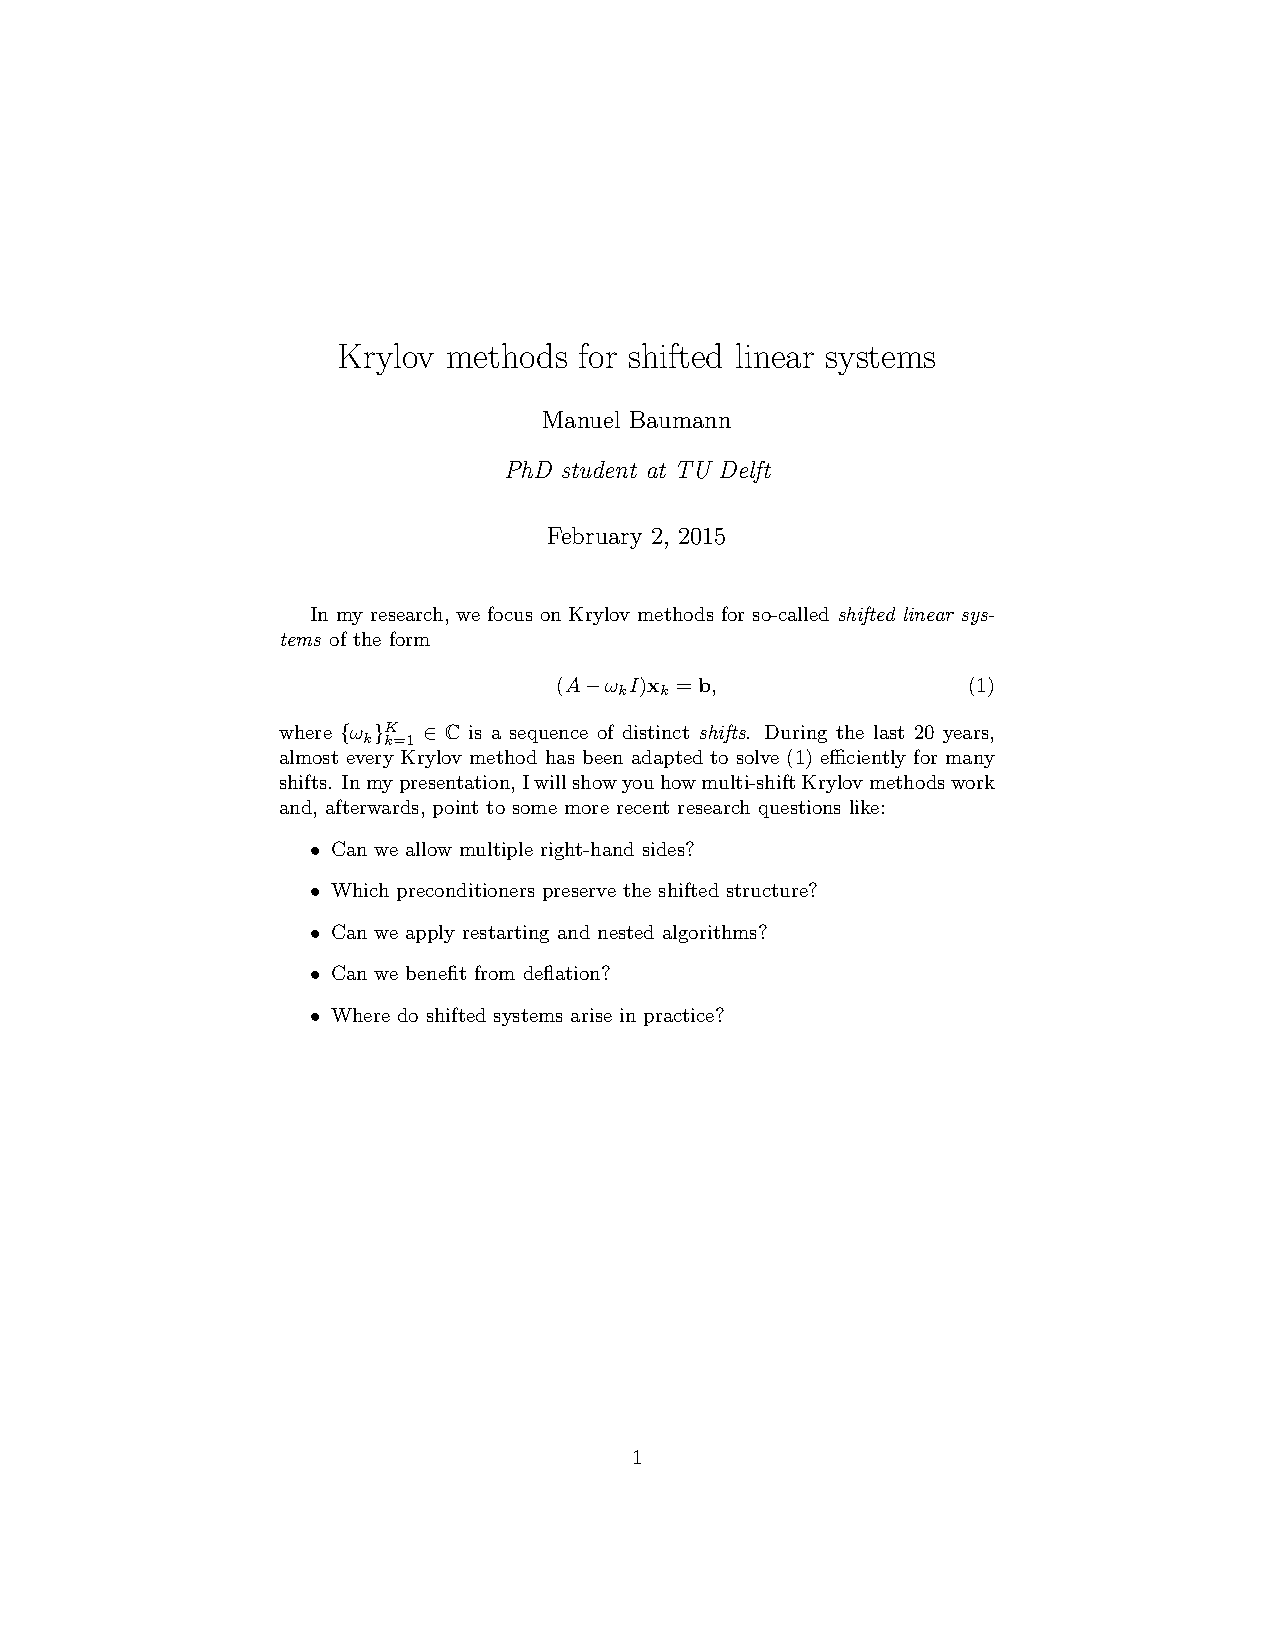
\includepdf[pages={1}]{abstracts/baumann_kd15.pdf}
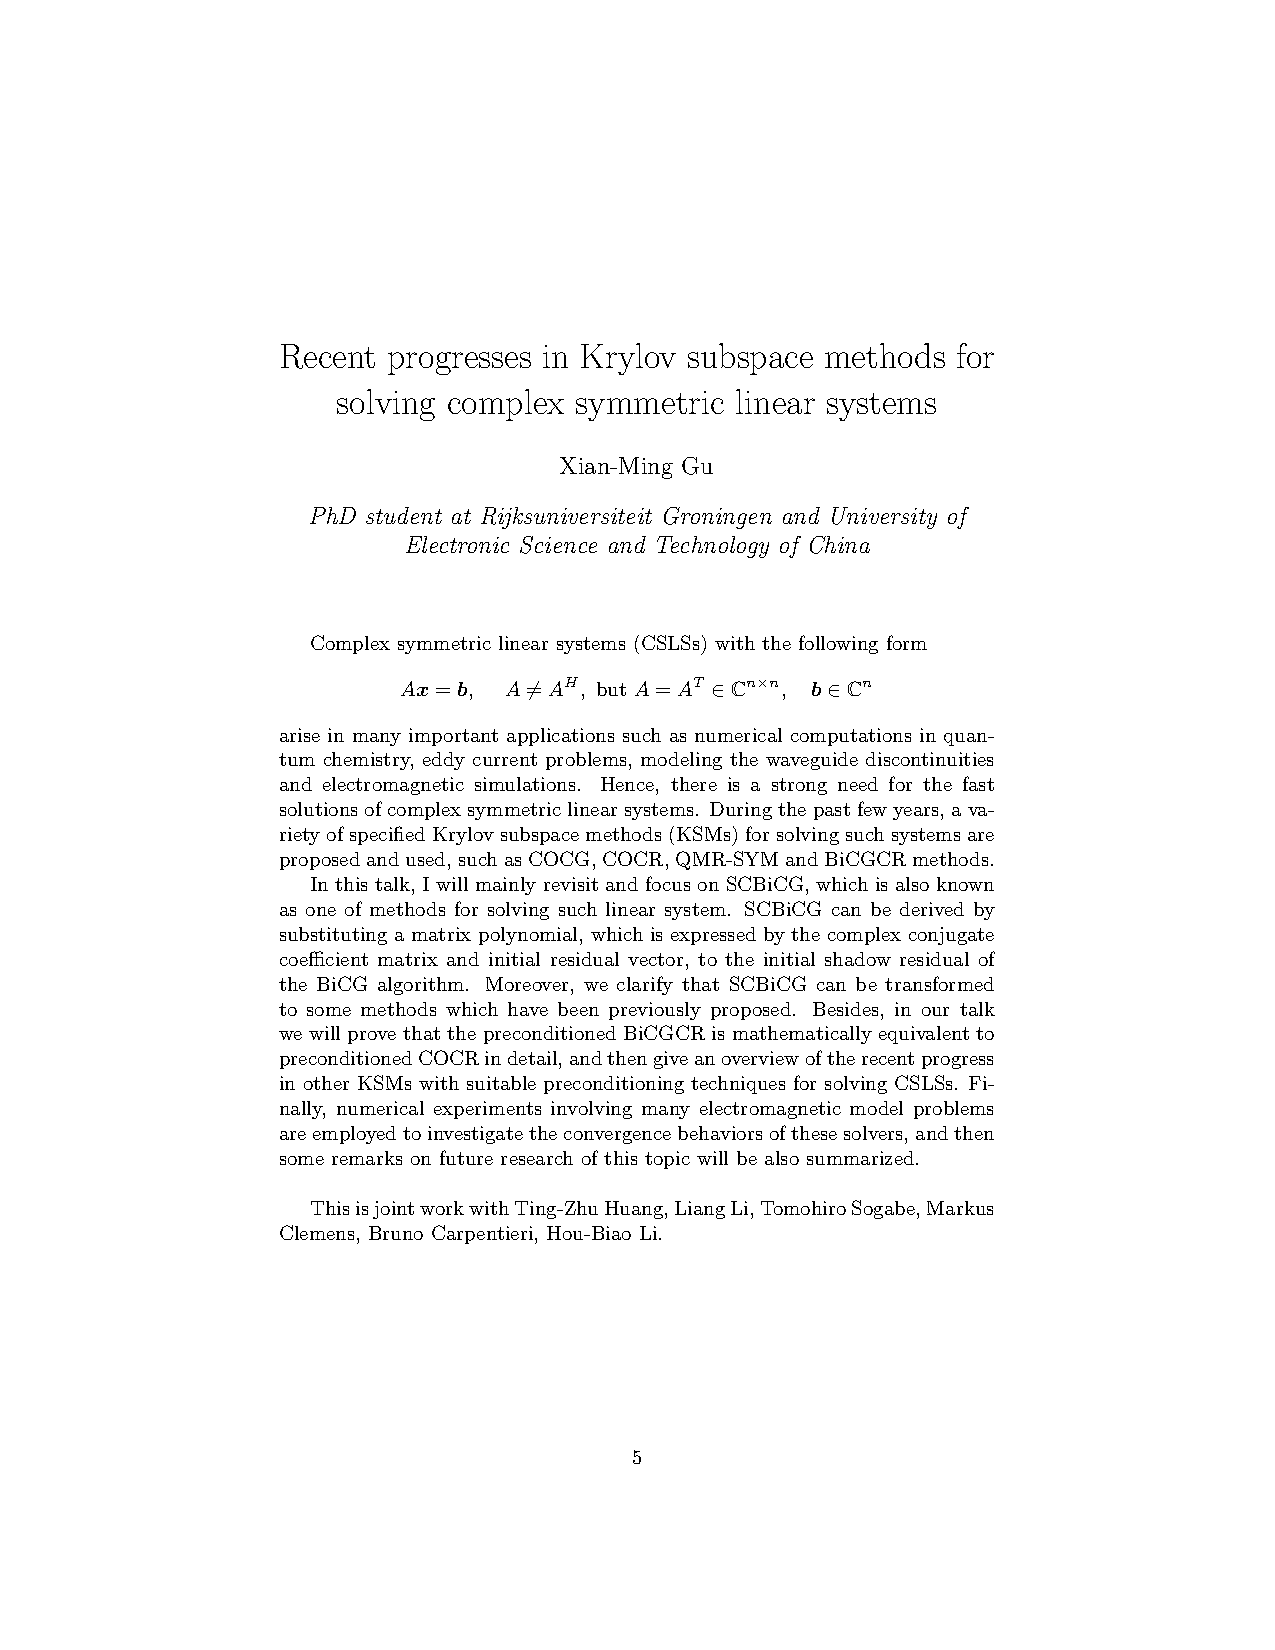
\includepdf[pages={1}]{abstracts/gu_kd_template.pdf}
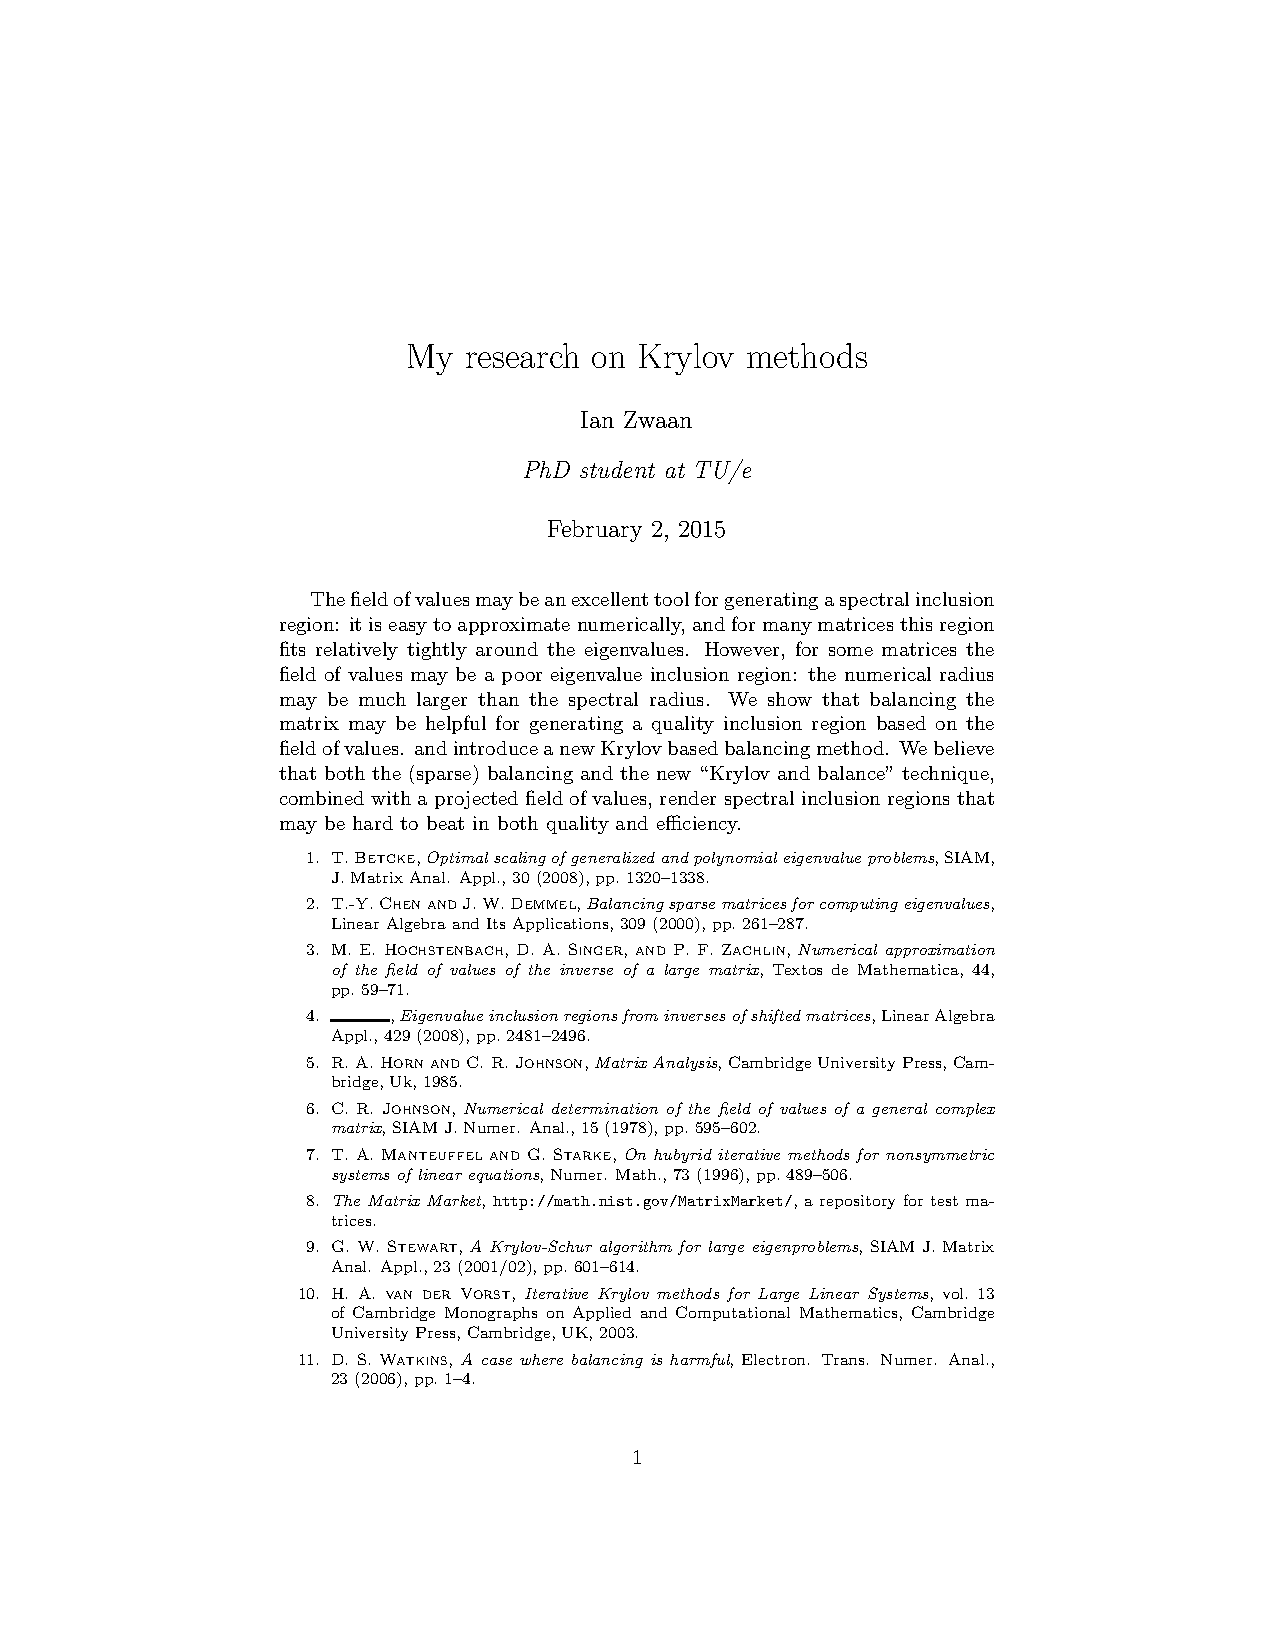
\includepdf[pages={1}]{abstracts/zwaan_kd15_template.pdf}
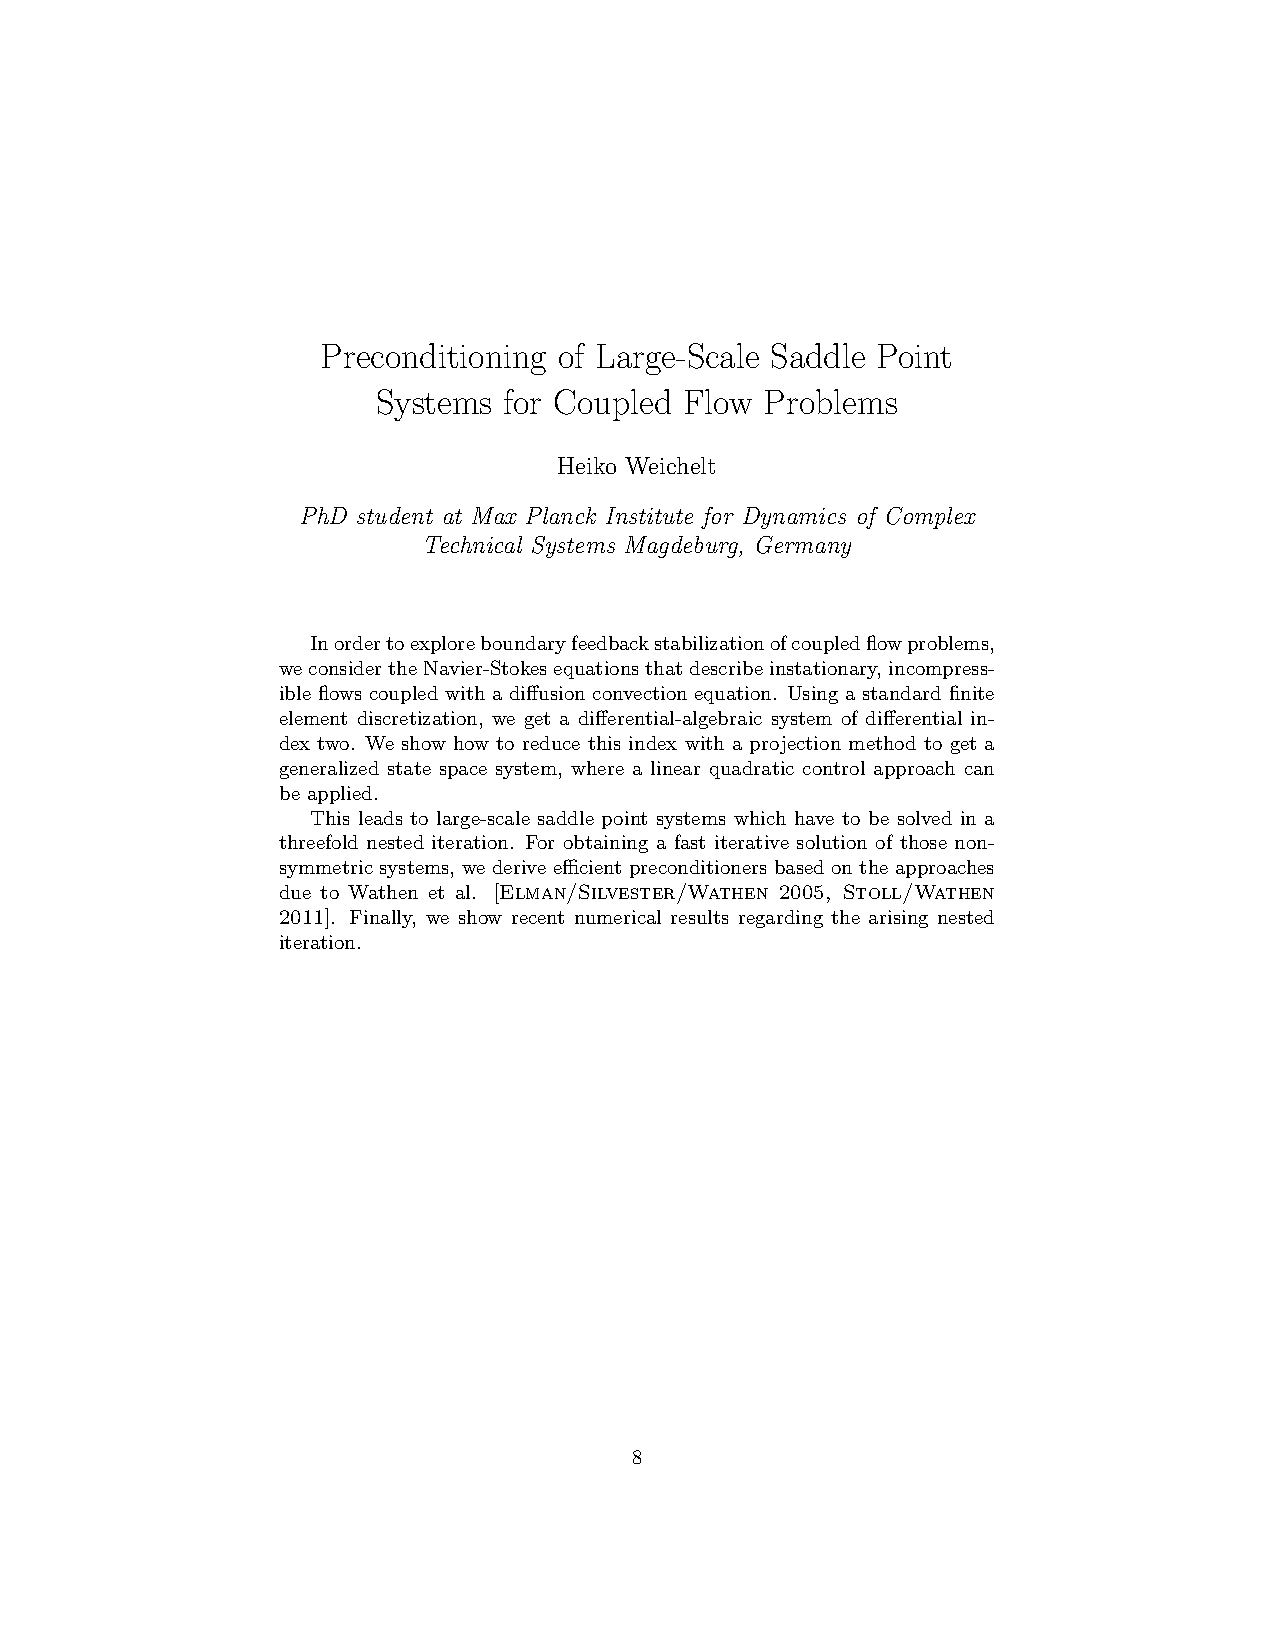
\includepdf[pages={1}]{abstracts/weichelt_abstract_KrylovDay_2015.pdf}
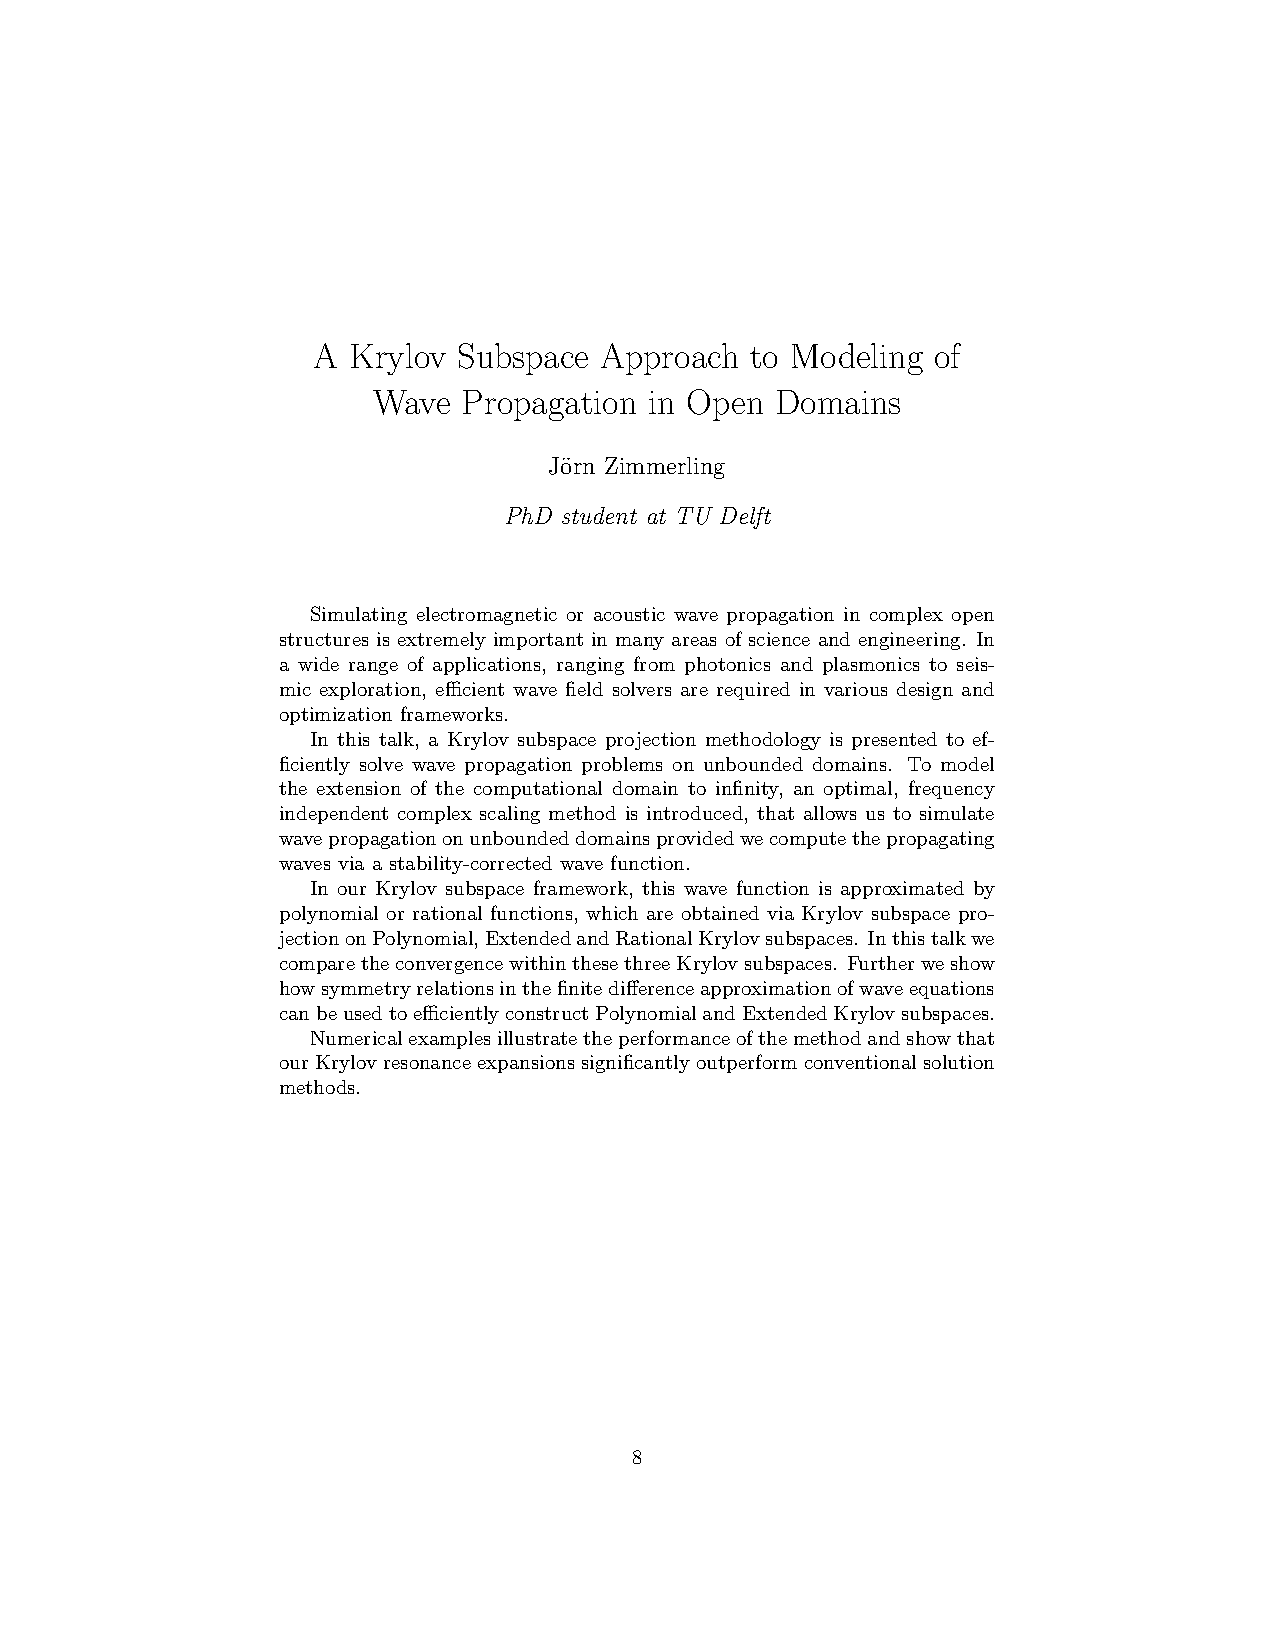
\includepdf[pages={1}]{abstracts/kd_jtzimmerling.pdf}
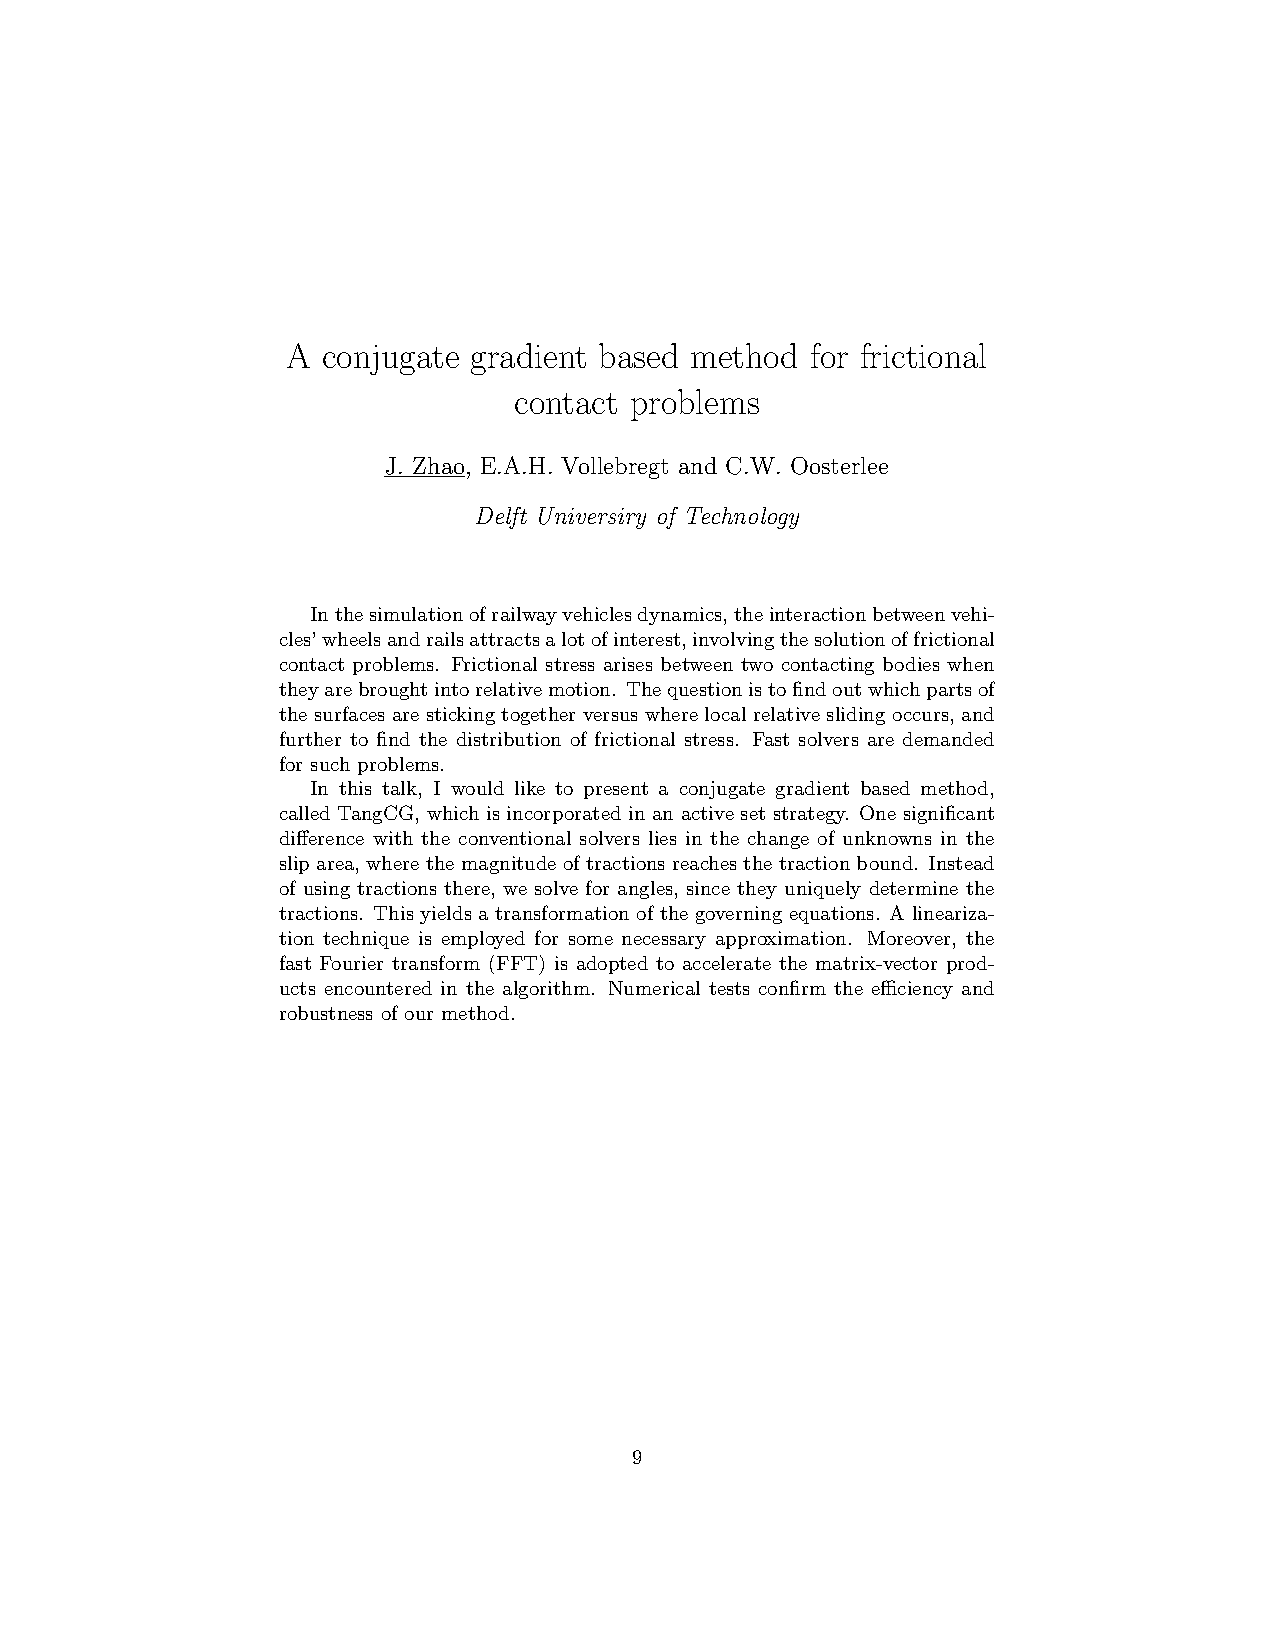
\includepdf[pages={1}]{abstracts/jing_kd_template.pdf}
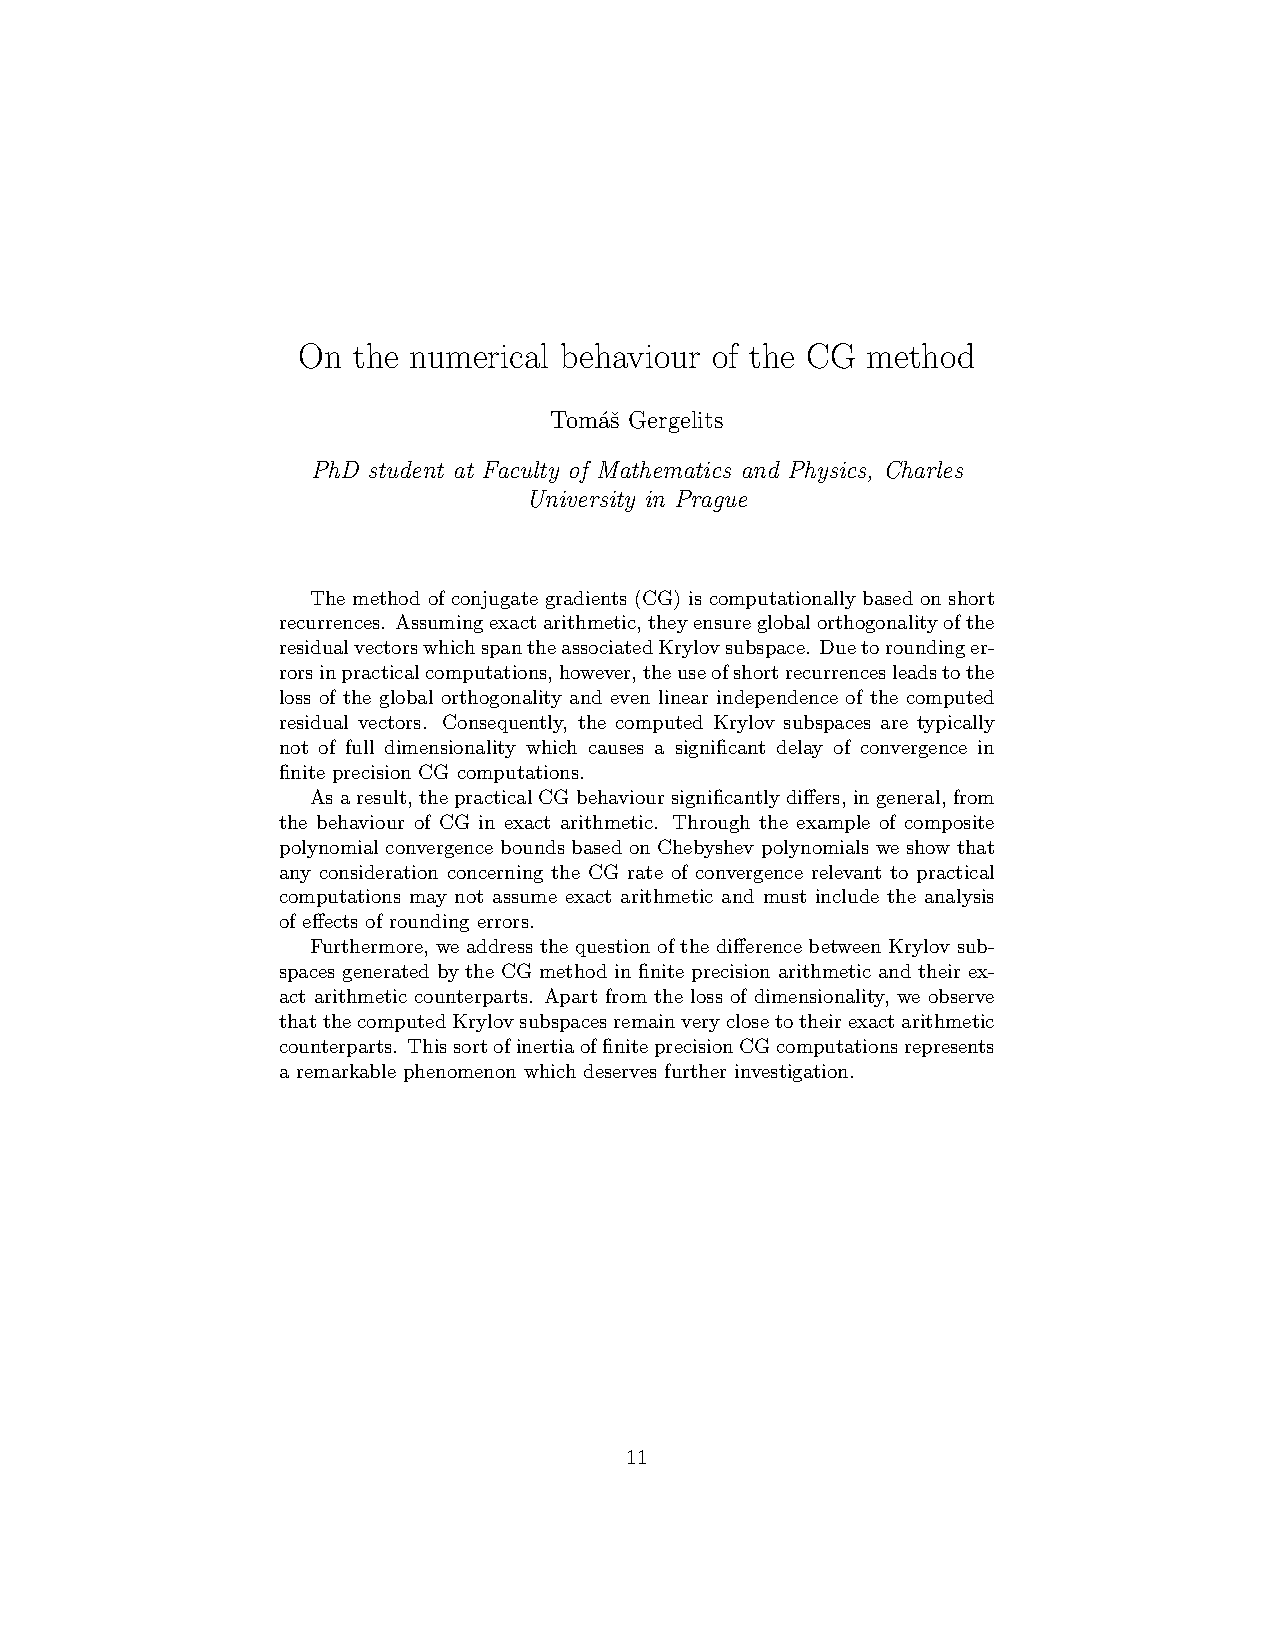
\includepdf[pages={1}]{abstracts/kd15_gergelits.pdf}
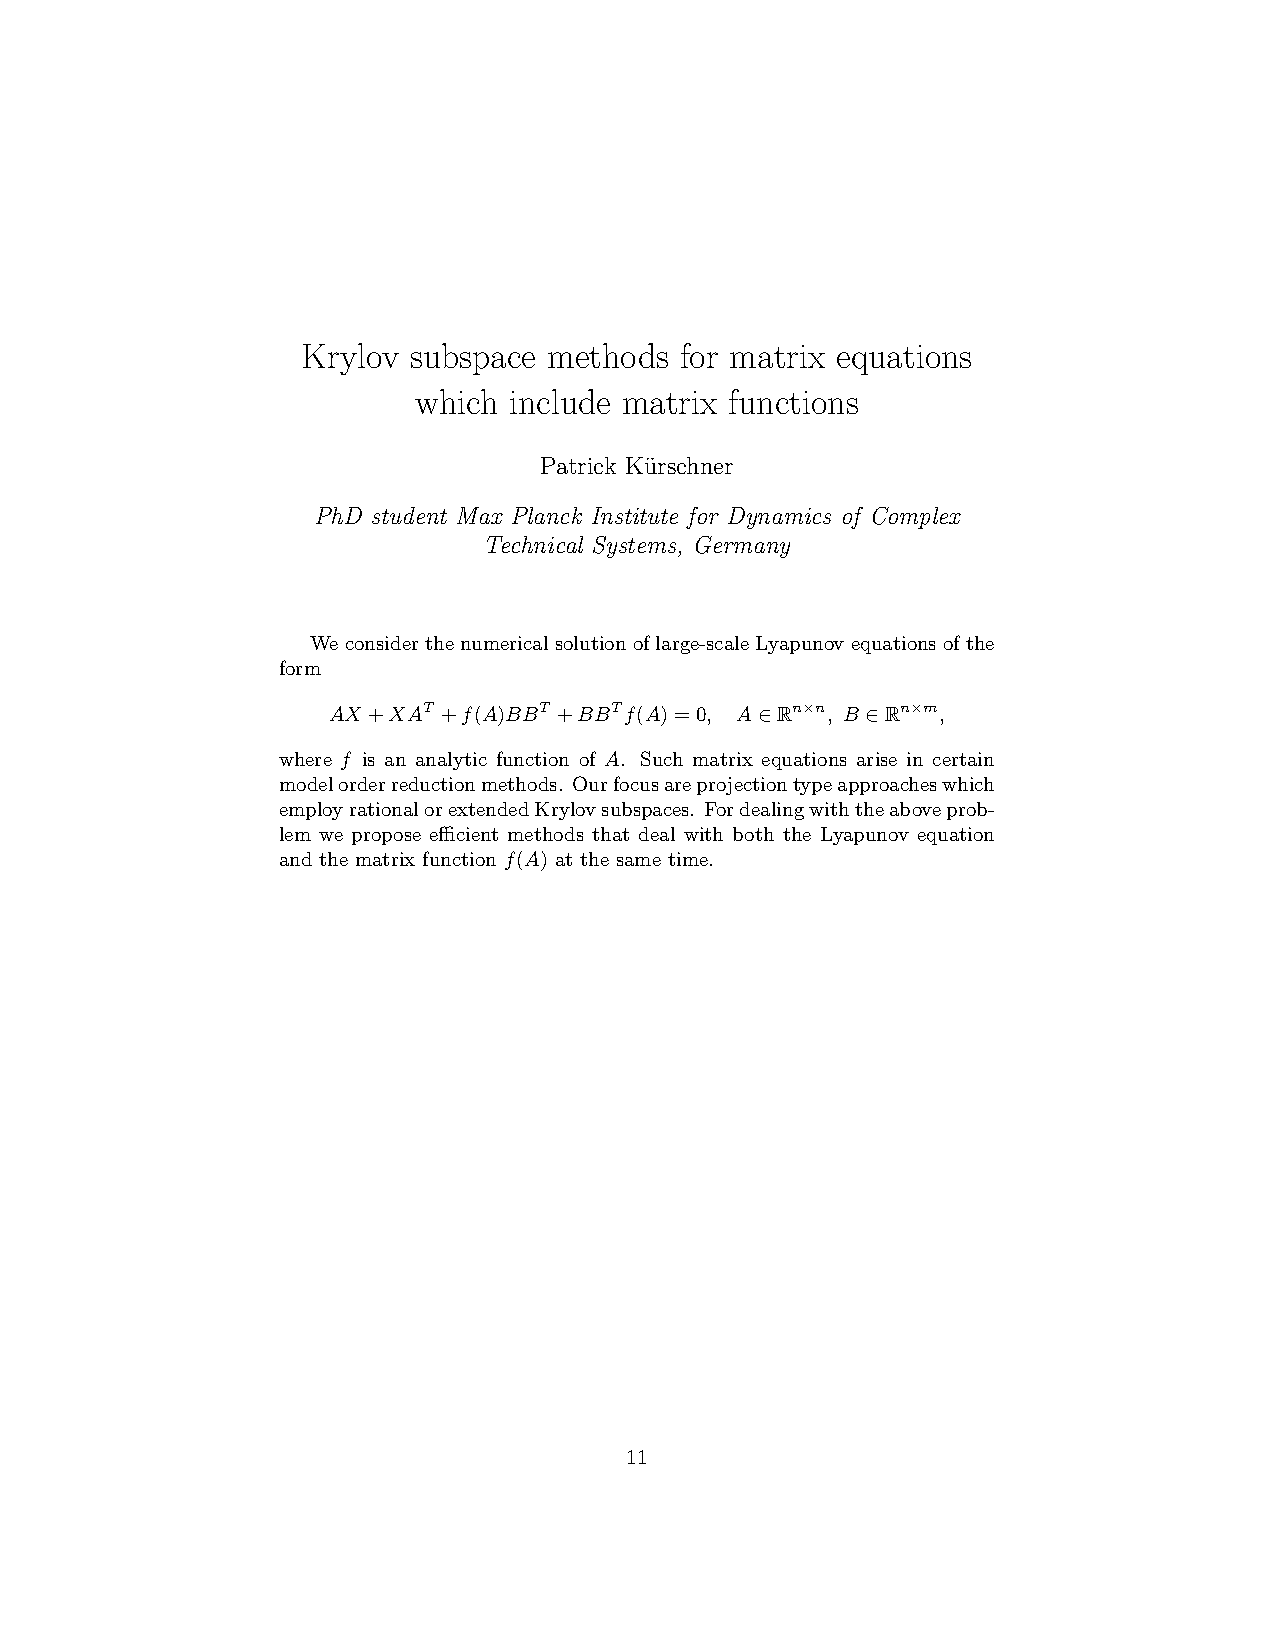
\includepdf[pages={1}]{abstracts/abstract_kuerschner.pdf}
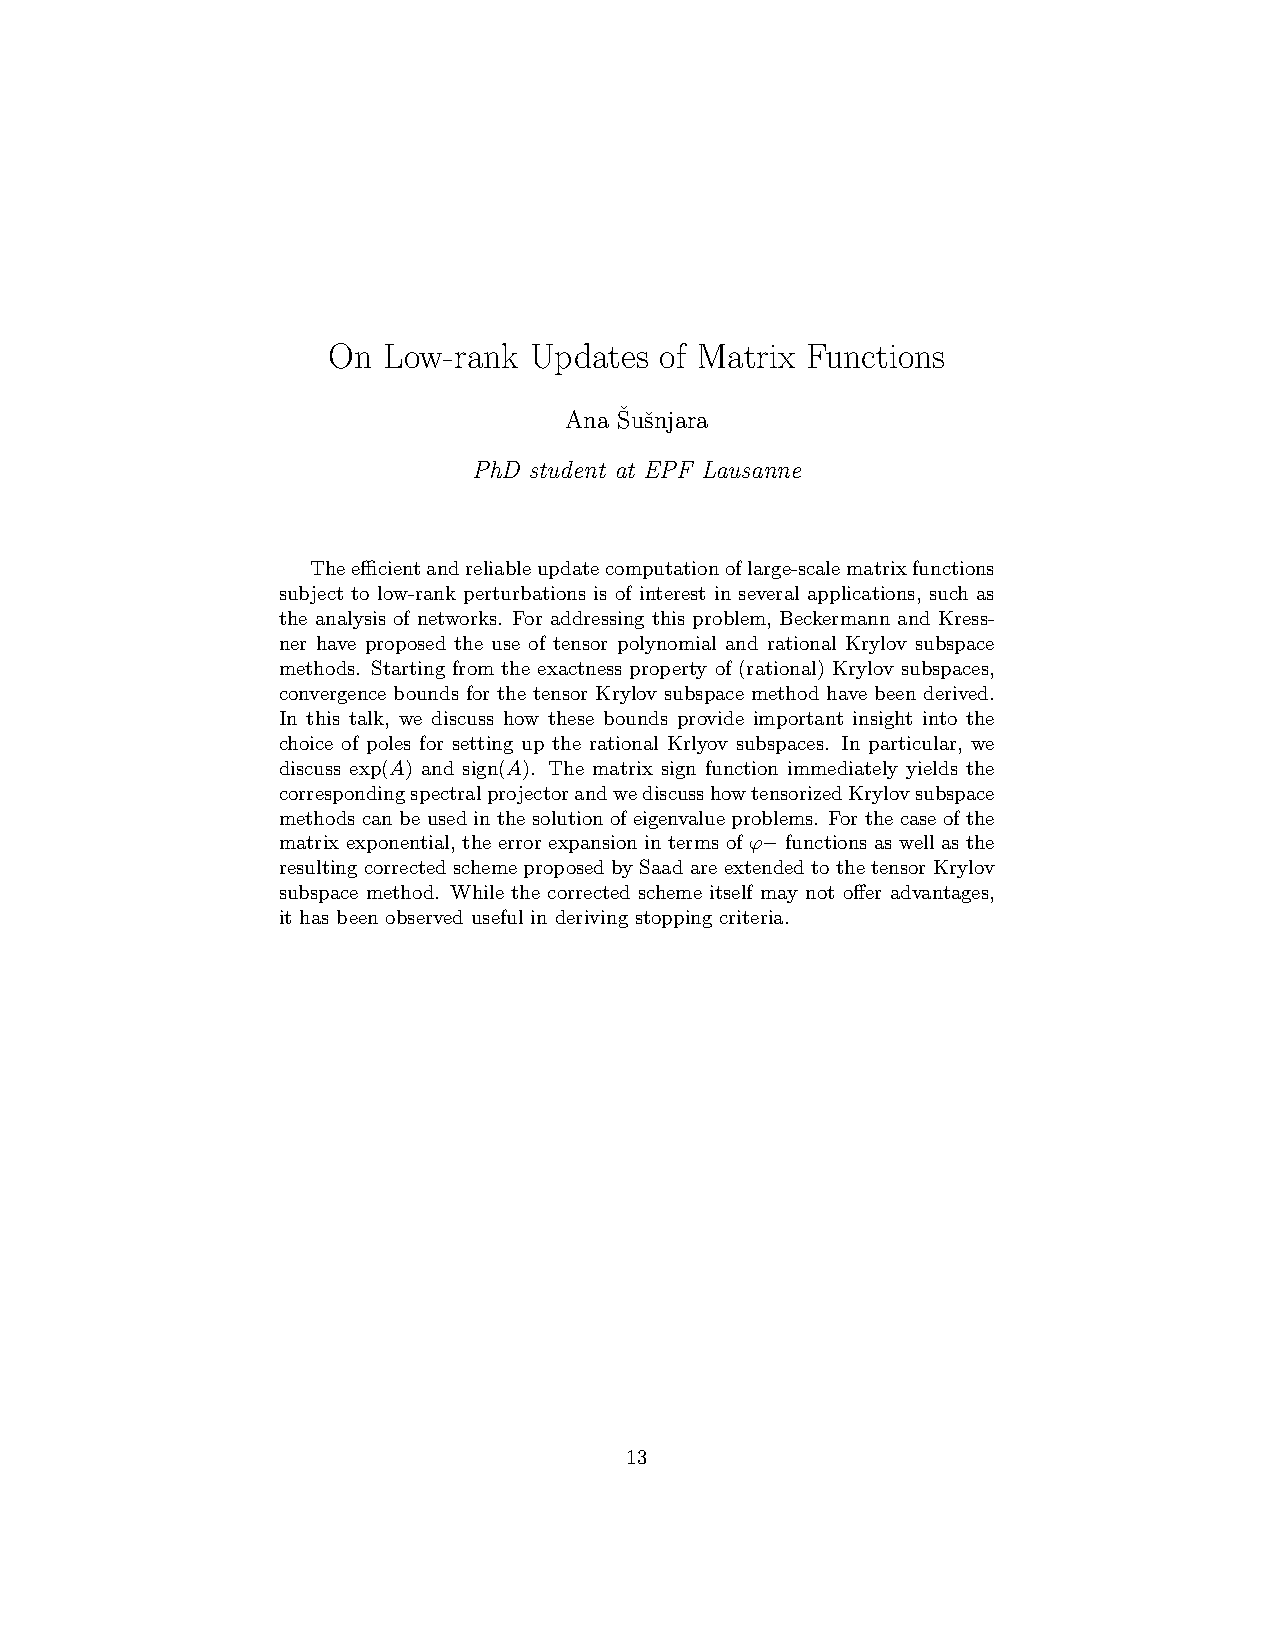
\includepdf[pages={1}]{abstracts/susnjara_template.pdf}
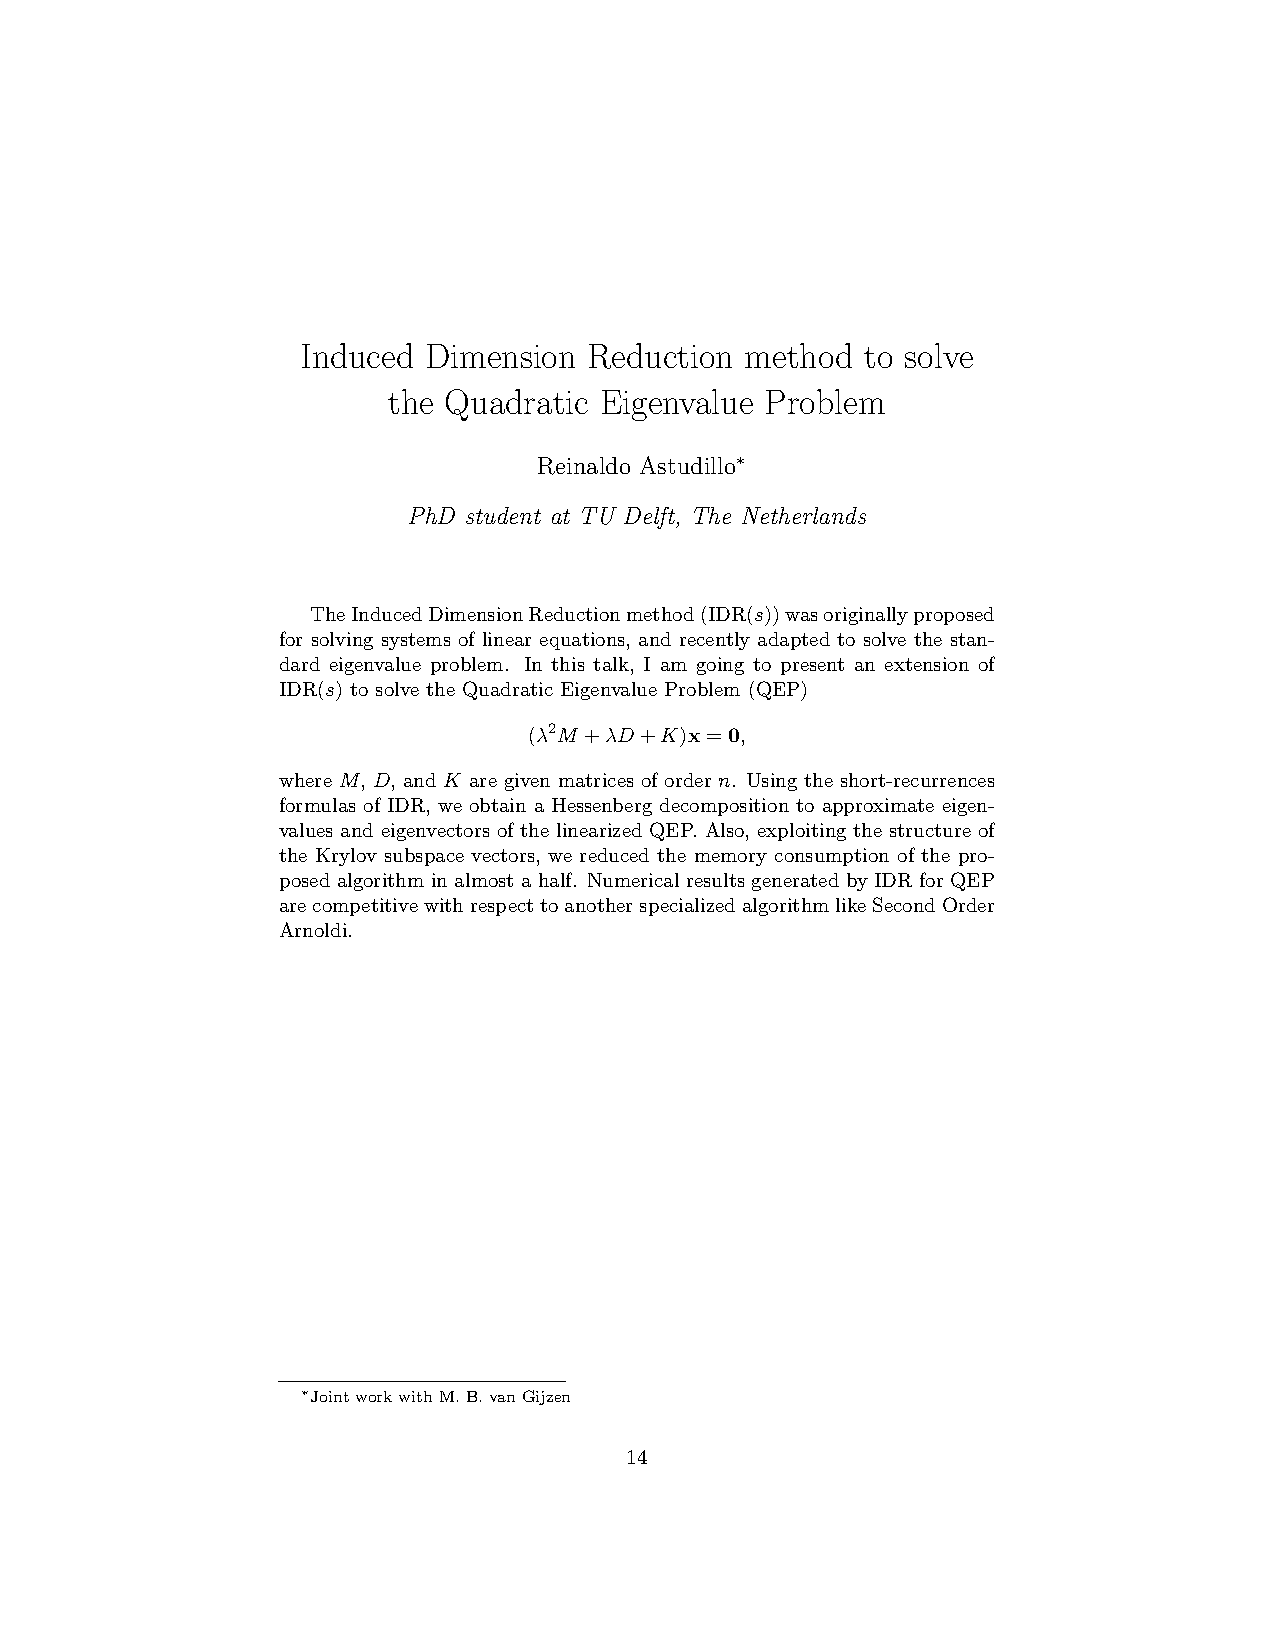
\includepdf[pages={1}]{abstracts/kd_template_Reinaldo.pdf}
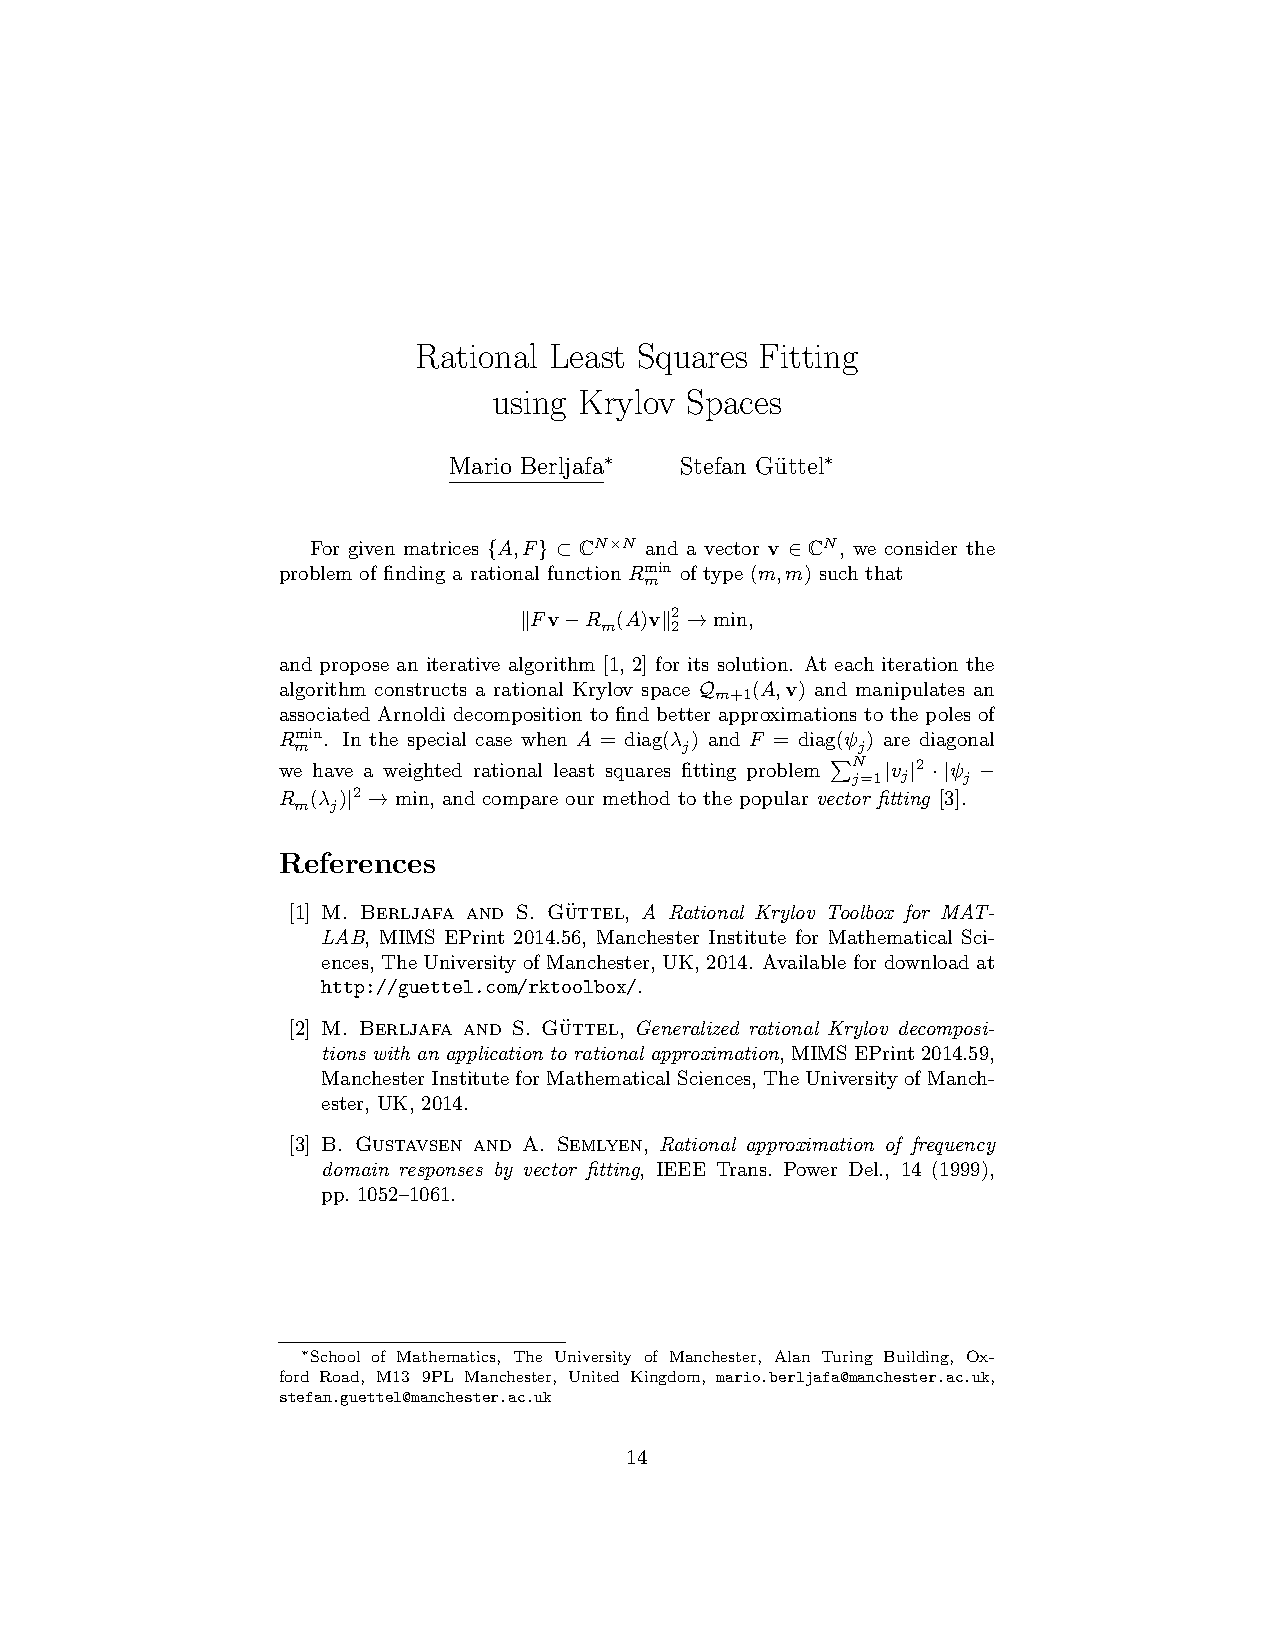
\includepdf[pages={1}]{abstracts/kd_berljafa.pdf}
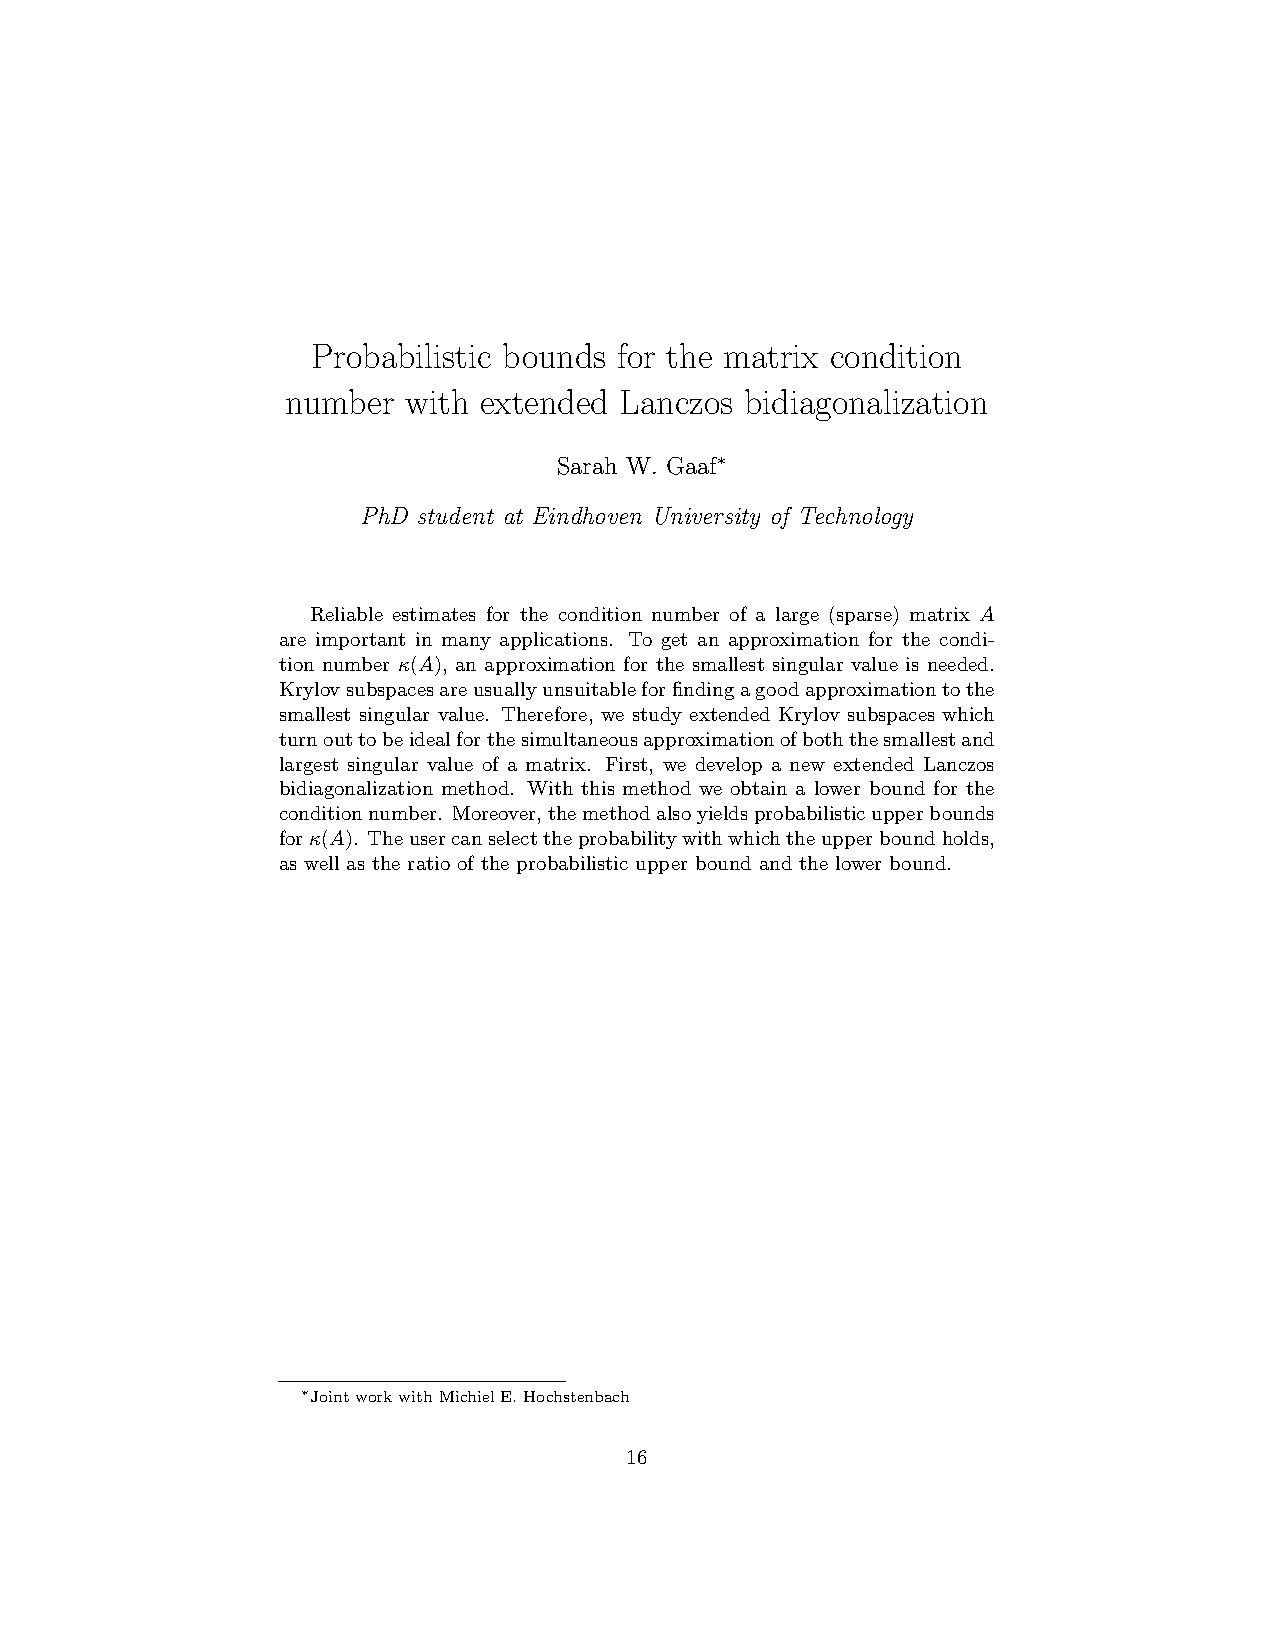
\includepdf[pages={1}]{abstracts/kd15_SarahGaaf.pdf}
\newpage
\noindent\large{\textbf{Email Directory}}
\begin{table}[h!]
 \centering
\begin{tabular}{|l|l|l|}
 \hline
\textbf{Name} & \textbf{University} & \textbf{Email address} \\
\hline
Reinaldo Astudillo & TU Delft & \href{mailto:R.A.Astudillo@tudelft.nl}{R.A.Astudillo@tudelft.nl} \\
\hline
Manuel Baumann & TU Delft & \href{mailto:M.M.Baumann@tudelft.nl}{M.M.Baumann@tudelft.nl} \\
\hline
Mario Berljafa & University of Manchester & \href{mailto:mario.berljafa@manchester.ac.uk}{mario.berljafa@manchester.ac.uk} \\
\hline
Sarah Gaaf & TU Eindhoven & \href{mailto:s.w.gaaf@tue.nl}{s.w.gaaf@tue.nl} \\
\hline
Tom{\'a}{\v s} Gergelits & Charles University, Prague & \href{mailto:gergelits@karlin.mff.cuni.cz}{gergelits@karlin.mff.cuni.cz} \\
\hline
Xian-Ming Gu & Rijksuniversiteit Groningen  & \href{mailto:x.m.gu@rug.nl}{x.m.gu@rug.nl} \\
&and UESTC, China & \\
\hline
Patrick K\"{u}rschner & MPI Magdeburg & \href{mailto:kuerschner@mpi-magdeburg.mpg.de}{kuerschner@mpi-magdeburg.mpg.de} \\
\hline
Peter Sonneveld & TU Delft &\href{mailto:P.Sonneveld@tudelft.nl}{P.Sonneveld@tudelft.nl} \\
\hline
Ana {\v S}u{\v s}njara & EPFL, Lausanne & \href{mailto:ana.susnjara@epfl.ch}{ana.susnjara@epfl.ch} \\
\hline
Heiko Weichelt & MPI Magdeburg & \href{mailto:weichelt@mpi-magdeburg.mpg.de}{weichelt@mpi-magdeburg.mpg.de}\\
\hline
Jing Zhao & TU Delft & \href{mailto:J.Zhao-1@tudelft.nl}{J.Zhao-1@tudelft.nl} \\
\hline
J\"orn Zimmerling & TU Delft &\href{mailto:jtzimmerling@gmail.com}{jtzimmerling@gmail.com} \\
\hline
Ian Zwaan & TU Eindhoven &\href{mailto:i.n.zwaan@tue.nl}{i.n.zwaan@tue.nl} \\
\hline
\end{tabular}
\end{table}

\bigskip
We will tweet about the workshop using the account \texttt{@SSC\_Delft} and hashtag \texttt{\#KD15}.

\vfill

\begin{center}
 \href{http://sscdelft.github.io/}{http://sscdelft.github.io/}
\end{center}


\end{document}
